\documentclass{article}
\usepackage[utf8]{inputenc}
\usepackage{titling}
\usepackage{graphicx}
\usepackage{xcolor}
\usepackage[colorlinks=true,linkcolor=darkgray, urlcolor =gray]{hyperref}
\usepackage[spanish]{babel}
\DeclareUnicodeCharacter{301}{~}
\newcommand\tab[1][1cm]{\hspace*{#1}}
\usepackage{url}


\title{Práctica 8. Control difuso con Qtfuzzylite}
\author{Cristina Díaz García}
\date{Mayo 2019}

\renewcommand\maketitlehooka{\null\mbox{}\vfill}
\renewcommand\maketitlehookd{\vfill\null}


\begin{document}

\addcontentsline{toc}{section}{Índice general}

\begin{titlingpage}
\maketitle
\end{titlingpage}

\newpage

\tableofcontents

\newpage

\section{Enunciado}

\textbf{\underline{Tarea:}} Contesta a las preguntas que figuran a continuación

\textbf{\underline{Entrega:}} Documento pdf con la solución (capturas de pantalla y textos descriptivos)

\section{Pregunta 1}

En el problema del tutorial, considera ahora las siguientes funciones: suma drástica (unión); producto
drástico (intersección), regla max-prod (para activar la regla) y método del centroide para decodificar. Captura la
última pantalla, y compara con los resultados con los obtenidos en el tutorial.
Para los siguientes problemas que resolvimos ayer en clase, impleméntalos en Qtfuzzylite. Describe los pasos de la
inferencia, incluyendo capturas de pantalla. Si la aplicación da errores respecto a la solución de clase, coméntalos.

\subsection{Solución proporcionada}

Los resultados del tutorial:

\begin{center}
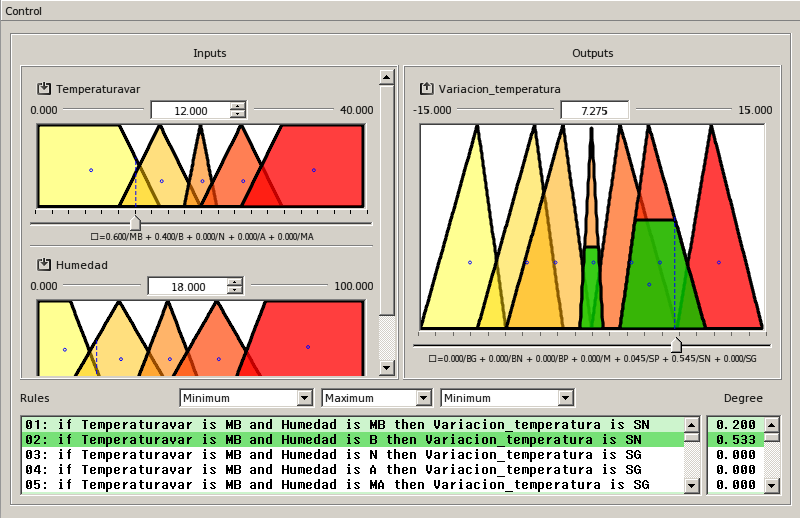
\includegraphics[scale=0.5]{images/res1.png}
\end{center}

\newpage

Los resultados del ejercicio:

\begin{center}
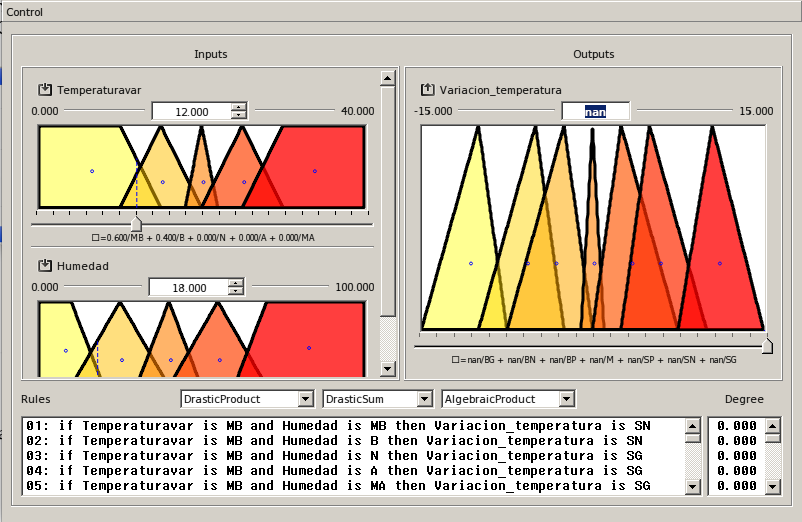
\includegraphics[scale=0.5]{images/res2.png}
\end{center}

Como se puede comprobar, en el tutorial obtenemos como solución 7.275, mientras que en el ejercicio no obtenemos solución.

\section{Pregunta 2}

La abuela María prepara sus deliciosas galletas caseras de forma artesanal desde hace más de 40 años.
El toque secreto de la receta consiste en hornearlas cuidadosamente de acuerdo a las siguientes reglas:

R1. Si las galletas están un poco crudas, entonces la temperatura del horno debe ser alta.

R2. Si las galletas están medio hechas, entonces la temperatura del horno debe ser media.

R3. Si las galletas están doraditas, entonces la temperatura del horno debe ser baja.

Tras diversas entrevistas con la abuela se han podido establecer los siguientes conjuntos difusos sobre un índice cromático especial (0 = galleta cruda; 10 = galleta chamuscada) y la temperatura del horno:

Índice cromático de las galletas:\\
\tab \textit{un poco crudas: (1/4, 0.5/6, 0/7)} \\
\tab \textit{medio hechas: (0/3, 1/5, 1/6, 0/8)} \\
\tab \textit{doraditas: (0/5, 1/7)} 

Temperatura del horno (ºC):\\
\tab \textit{baja: (0/150, 1/160, 1/180, 0/190)} \\
\tab \textit{media: (0/170, 1/190, 1/210, 0/230)} \\
\tab \textit{alta: (0/210, 1/220, 1/240, 0/250)} \\
Supóngase que se interpretan las reglas anteriores como implicaciones de Mamdani. Suponiendo que en cierto momento el índice cromático de las galletas es 6, ¿Cuál será el valor de temperatura aplicado al horno si se utiliza la técnica del primer valor máximo para obtener valores nítidos?

\subsection{Solución proporcionada}

\begin{center}
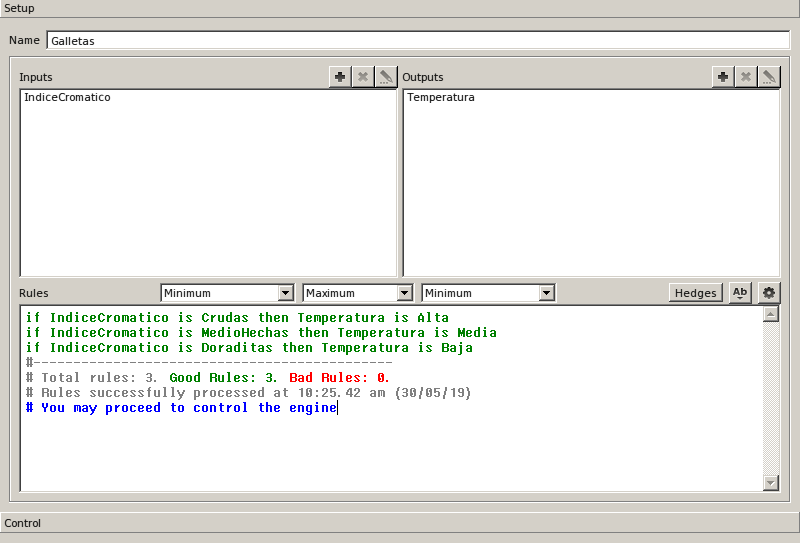
\includegraphics[scale=0.5]{images/ej2.png}
\end{center}

\begin{center}
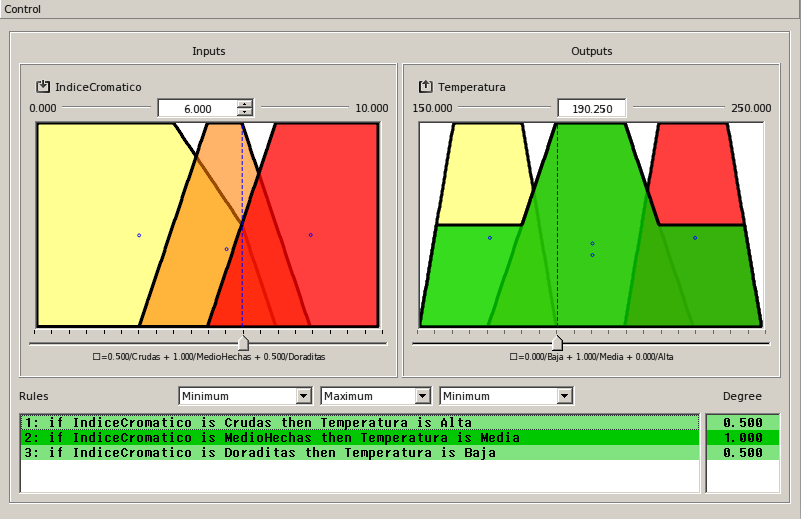
\includegraphics[scale=0.5]{images/ej22.png}
\end{center}

El valor que nos da es 190.250 ºC, aunque al hacerlo en papel nos dio 190 ºC.

\section{Pregunta 3}

Considérese un sistema con las siguientes reglas, interpretadas como implicaciones de Mamdani:

R1. Si la temperatura es alta entonces la presión es elevada.

R2. Si la temperatura es baja entonces la presión es baja.

R3. Si la presión es baja entonces la entrada de combustible debe ser grande.

R4. Si la presión es elevada entonces la entrada de combustible debe ser pequeña.

Con los siguientes conjuntos difusos:

Temperatura(ºC):\\
\tab \textit{baja = (0/0 .2/30 .8/40 1/50 .7/60 .2/70 0/80)}\\
\tab \textit{alta = (0/50 .3/60 .8/70 1/80 1/90 .5/100 0/110)}

Presión(bar):\\
\tab \textit{baja = (0/0 .4/200 .8/400 1/600 1/800 .8/1000 .4/1200 0/1400)}\\
\tab \textit{Elevada = (0/1000 .2/1200 .4/1400 .8/1600 1/1800 1/1900 .5/2000 0/2200)}

Entrada combustible(litros/hora):\\
\tab \textit{pequeña = (0/0 .6/1 1/2 1/3 .4/4 0/5)}\\
\tab \textit{grande = (0/4 .5/5 1/6 .5/7 0/8)}\\
Si la temperatura actual es 60ºC, determina el valor para la entrada de combustible empleando la técnica del primer valor máximo para transformar valores difusos en nítidos

\subsection{Solución proporcionada}

\begin{center}
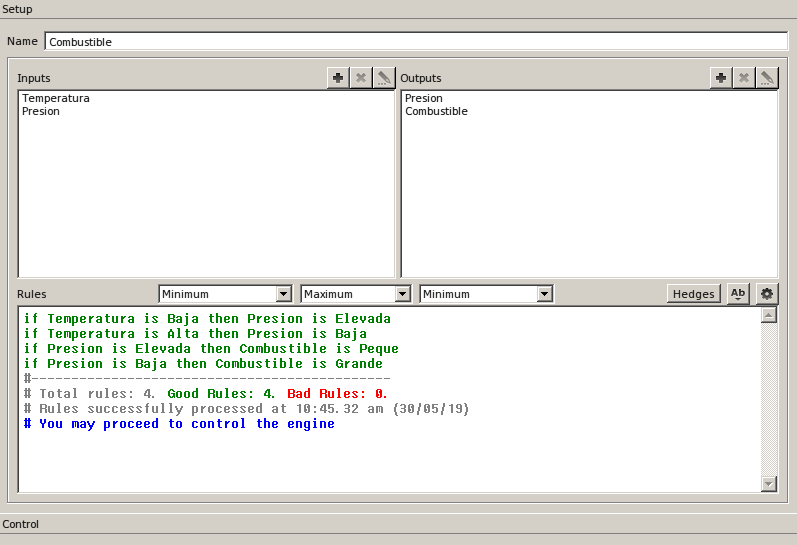
\includegraphics[scale=0.5]{images/ej3.png}
\end{center}

\begin{center}
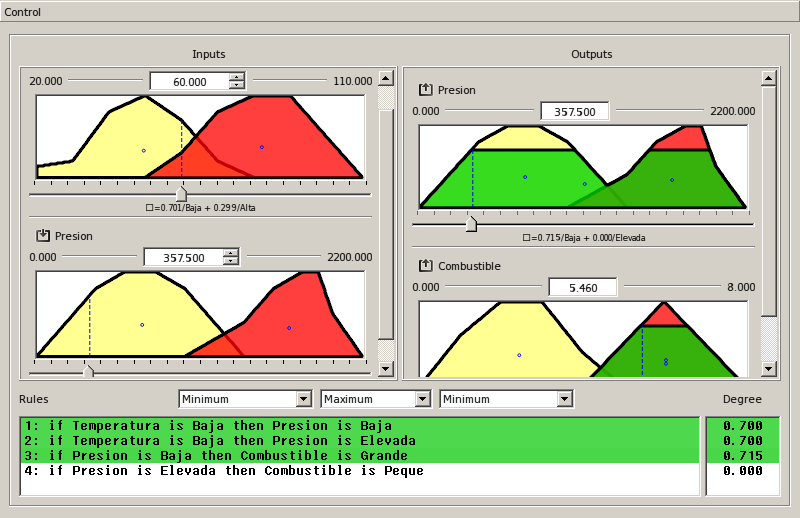
\includegraphics[scale=0.5]{images/ej32.png}
\end{center}

La salida sería 5.460 L/h, aunque al hacerlo en papel nos dio 5.5 L/h.

\section{Pregunta 4}

Agapito lleva 8 años encargado del control de la turbina GG-35 y es ya una autoridad en su manejo. Agapito ha reconocido que para controlar la turbina solamente
se fija en el ruido que produce y en un sensor de temperatura:

R1. Si el nivel de ruido es normal y la temperatura es alta, entonces establece una velocidad suave.

R2. Si el nivel de ruido es normal y la temperatura no es alta, entonces establece una velocidad moderada.

R3. Si el nivel de ruido es bajo, entonces establece una velocidad alta.

R4. Si la velocidad es suave, la fuerza de frenado debe ser normal.

R5. Si la velocidad es moderada, la fuerza de frenado debe ser alta.

R6. Si la velocidad es alta, la fuerza de frenado debe ser alta.

Tras diversas entrevistas con Agapito se han elaborado los siguientes conjuntos difusos para los valores del nivel de ruido, temperatura, velocidad y fuerza de frenado:

Nivel de ruido (escala 0 a 12):\\
\tab \textit{bajo (0/1, 1/3, 1/5, 0/7)}\\
\tab \textit{normal (0/5, 1/7, 1/9, 0/11)}

Temperatura (escala 20º-100ºC):\\
\tab \textit{alta (0/40, 1/60, 0/80)}

Velocidad (escala 0 a 100 rpm):\\
\tab \textit{suave (0/10, 1/30, 0/50)}\\
\tab \textit{moderada (0/30, 1/50, 0/70)}\\
\tab \textit{alta (0/40, 0.5/50, 0.5/60, 1/70, 0.5/80, 0.5/90, 0/100)}

Fuerza de frenado (escala 0 a 5):\\
\tab \textit{normal (0/1, 1/3, 0/5)}\\
\tab \textit{alta (0/3, 1/4)}\\
Suponiendo que en cierto momento el nivel de ruido es 5,5 y la temperatura de 50ºC, calcula el valor de la fuerza de frenado si se utiliza la técnica de la media de los valores máximos para obtener valores nítidos.

\subsection{Solución proporcionada}

\begin{center}
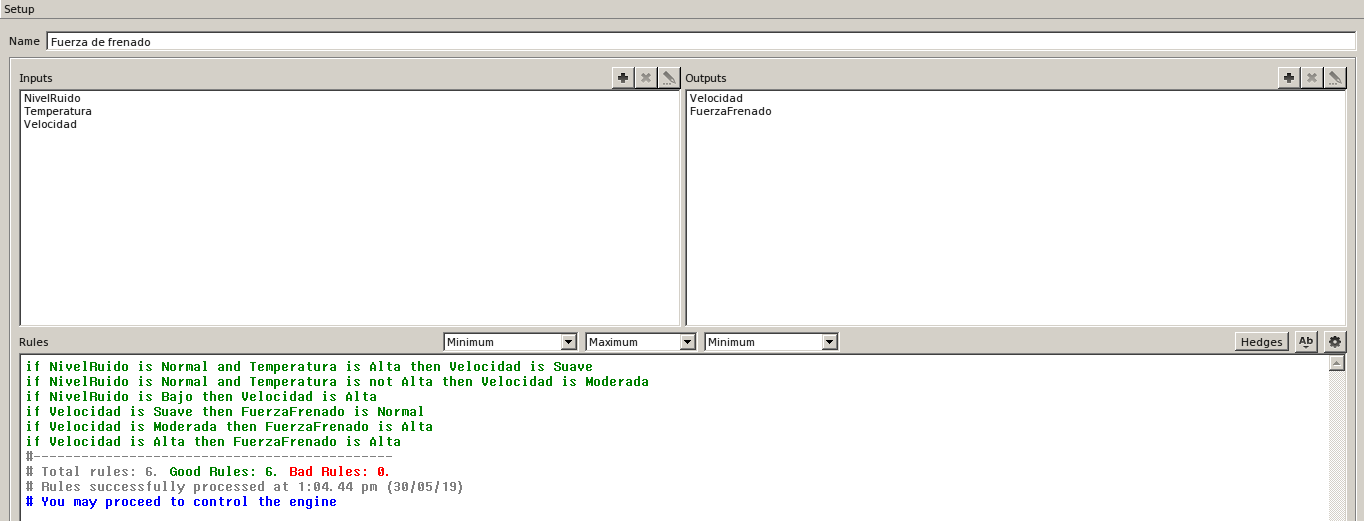
\includegraphics[scale=0.3]{images/ej4.png}
\end{center}

\begin{center}
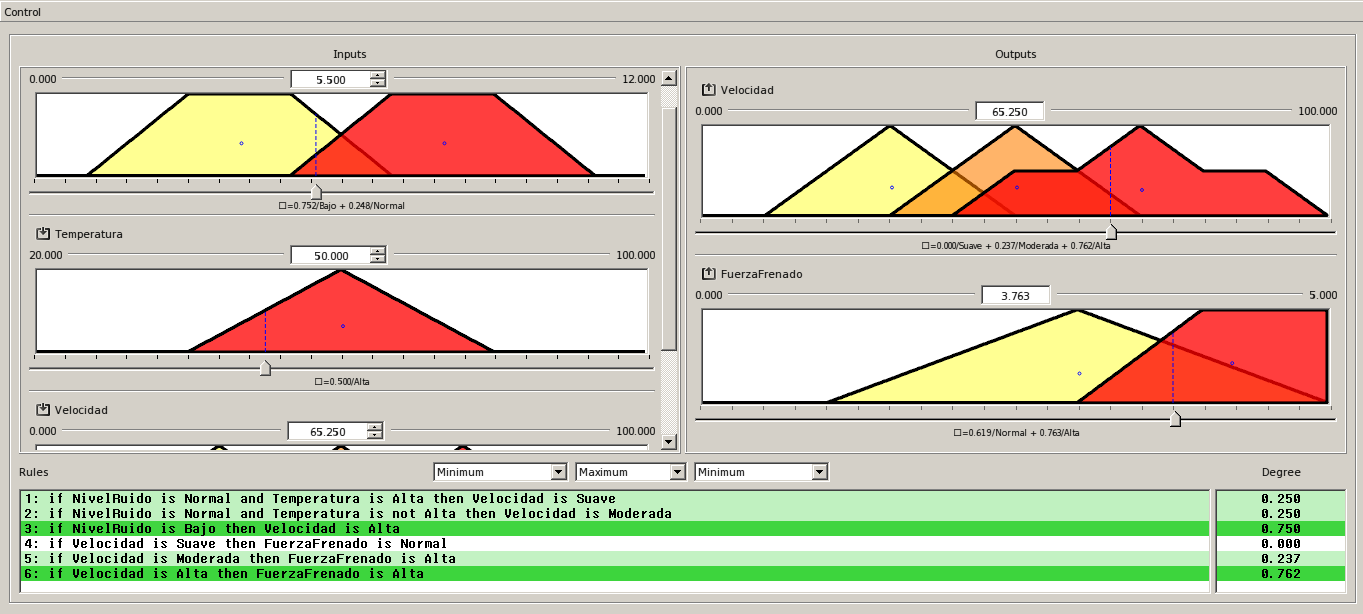
\includegraphics[scale=0.3]{images/ej42.png}
\end{center}

La fuerza de frenado sería 3.763

\begin{thebibliography}{9}
\bibitem{Bayes} Información oficial de GeNIe, \url{https://www.bayesfusion.com}.
\end{thebibliography}

\end{document}